\chapter{图}
在ACM竞赛中,图一般使用邻接矩阵表示,代码框架如下;

\begin{Codex}[label=graph.cpp ]
#define MAXN 100  // 顶点最大个数

static int n; // 顶点个数
static int G[MAXN][MAXN]; // 邻接矩阵
static int visited_edges[MAXN][MAXN]; // 边的访问历史记录
static int visited_vertices[MAXN]; // 顶点的访问历史记录
\end{Codex}

\section{深度优先搜索} %%%%%%%%%%%%%%%%%%%%%%%%%%%%%%
图的深度优先搜索的代码框架如下:

\begin{Codex}[label=graph.cpp]
/**
 * @brief 图的深度优先搜索代码框架,搜索边.
 * @param[in] u 出发顶点
 * @param[in] n 顶点个数
 * @param[in] G 图的临街举着
 * @param[in] visited 边的访问历史记录
 * @return 无
 * @remark 在使用的时候,为了降低递归的内存占用量,可以把
 * n, G, visited 抽出来作为全局变量
 */
static void dfs(const int u, 
                const int n, const int G[][MAXN], int visited[][MAXN]) {
    int v;
    for(v = 0;  v < n; v++) if(G[u][v] && !visited[u][v]) {
        visited[u][v] = visited[v][u] = 1; // 无向图用这句
        // visited_edges[u][v] = 1; // 有向图用这句
        dfs(v, n, G, visited);
        // 这里写逻辑代码
        // printf("%d %d\n", u, v);
    }
}

/**
 * @brief 图的深度优先搜索代码框架,搜索顶点.
 * @param[in] u 出发顶点
 * @param[in] n 顶点个数
 * @param[in] G 图的临街举着
 * @param[in] visited 顶点的访问历史记录
 * @return 无
 * @remark 在使用的时候,为了降低递归的内存占用量,可以把
 * n, G, visited 抽出来作为全局变量
 */
static void dfs(const int u, 
                const int n, const int G[][MAXN], int visited[MAXN]) {  
    int v;
    visited[u] = 1;
    for(v = 0;  v < n; v++) if(G[u][v] && !visited[v]) {
        dfs(v, n, G, visited);
        // 这里写逻辑代码
        // printf("%d %d\n", u, v);
    }
}
\end{Codex}

\subsection{黑白图像}
输入一个n*n的黑白图像(1表示黑丝,0表示白色),任务是统计其中八连块的个数。
如果两个黑格子有公共边或者公共定点,就说它们属于同一个八连块。如图~\ref{fig:blackwhiteImage}所示的
黑白图像中有3个八连块。

\begin{center}
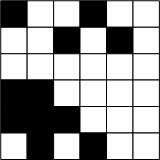
\includegraphics[width=90pt]{blackwhite-image.jpg}\\
\figcaption{拥有3个八连块的黑白图}\label{fig:blackwhiteImage}
\end{center}

\begin{Codex}[label=blackwhite_image.c]
#include <stdio.h>
#include <string.h>

#define MAXN 16

static int n;
// 黑白图,1 表示黑色,0表示白色,加一圈0,用于判断出界
static int G[MAXN + 1][MAXN + 1];
// 记录格子(x,y)是否已经被访问过
static int visitied[MAXN][MAXN];

void dfs(const int x, const int y) {
    // 曾经访问过这个格子,或者当前格子是白色
    if(G[x][y] == 0 || visitied[x][y] == 1)  return;
    
    visitied[x][y] = 1; // 标记(x,y)已访问过
    // 递归访问周围的8个格子
    dfs(x - 1, y - 1); // 左上角
    dfs(x - 1, y); // 正上方
    dfs(x - 1, y + 1); // 右上角
    dfs(x, y - 1); // 左边
    dfs(x, y + 1); // 右边
    dfs(x + 1, y - 1); // 左下角
    dfs(x + 1, y); // 正下方
    dfs(x + 1, y + 1); // 右下角
}

/*
Sample Input
6
100100
001010
000000
110000
111000
010100
Sample Output
3
*/
int main(int argc, char* argv[]) {
    int i, j;
    char s[MAXN]; // 矩阵的一行
    int count = 0; // 八连块的个数

    scanf("%d", &n);
    memset(G, 0, sizeof(G));
    memset(visitied, 0, sizeof(visitied));

    for(i = 0; i < n; ++i) {
        scanf("%s", s);
        for(j = 0; j < n; ++j) {
            G[i + 1][j + 1] = s[j] - '0'; // 把图像往中间挪一点,空出一圈白格子
        }
    }


    for(i = 1; i <= n; ++i) {
        for(j = 1; j <= n; ++j) {
            if(visitied[i][j] == 0 && G[i][j] == 1) {
                count++;
                dfs(i, j);
            }
        }
    }
    printf("%d\n", count);
    return 0;
}
\end{Codex}

\subsubsection{类似的题目}
与本题相同的题目:
\begindot
\item 《算法竞赛入门经典》\footnote{刘汝佳,算法竞赛入门经典,清华大学出版社,2009} 第107页6.4.1节
\item  TODO
\myenddot

与本题相似的题目:
\begindot
\item  TODO
\myenddot

\subsection{欧拉回路}
如果能从图的某一顶点出发,每条边恰好经过一次,这样的路线称为\textbf{欧拉道路}(Eulerian Path)。
如果每条边恰好经过一次,且能回到起点,这样的路线称为\textbf{欧拉回路}(Eulerian Circuit)。

对于无向图G,当且仅当G是连通的,且最多有两个奇点,则存在欧拉道路。
如果有两个奇点,则必须从其中一个奇点出发,到另一个奇点终止。

如果没有奇点,则一定存在一条欧拉回路。

对于有向图G,当且仅当G是连通的,且每个点的入度等于出度,则存在欧拉回路。

如果有两个顶点的入度与出度不相等,且一个顶点的入度比出度小1,另一个顶点的入度比出度大1,此时,
存在一条欧拉道路,以前一个顶点为起点,以后一个顶点为终点

\subsubsection{The Necklace} 
本题是 UVA 10054 - The Necklace。

My little sister had a beautiful necklace made of colorful beads. Two successive beads in the 
necklace shared a common color at their meeting point. The figure below shows a segment of 
the necklace:

\centerline{\fbox{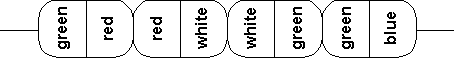
\includegraphics[width=240pt]{uva10054.png}}}

But, alas! One day, the necklace was torn and the beads were all scattered over the floor. 
My sister did her best to recollect all the beads from the floor, but she is not sure 
whether she was able to collect all of them. Now, she has come to me for help. She wants
 to know whether it is possible to make a necklace using all the beads she has in the same
 way her original necklace was made and if so in which order the bids must be put.

Please help me write a program to solve the problem.

\textbf{Input}

The input contains T test cases. The first line of the input contains the integer T.

The first line of each test case contains an integer $N(5 \leq N \leq 1000)$ giving the number of beads 
my sister was able to collect. Each of the next N lines contains two integers describing 
the colors of a bead. Colors are represented by integers ranging from 1 to 50.

\textbf{Output}

For each test case in the input first output the test case number as shown in the sample output. Then 
if you apprehend that some beads may be lost just print the sentence ``some beads may be lost" on a 
line by itself. Otherwise, print N lines with a single bead description on each line. Each bead 
description consists of two integers giving the colors of its two ends. For $1 \leq i \leq N_1$, the second integer 
on line i must be the same as the first integer on line i + 1. Additionally, the second integer 
on line N must be equal to the first integer on line 1. Since there are many solutions, any one
 of them is acceptable.

Print a blank line between two successive test cases.

\textbf{Sample Input} \\
2 \\
5 \\
1 2 \\
2 3 \\
3 4 \\
4 5 \\
5 6 \\
5 \\
2 1 \\
2 2 \\
3 4 \\
3 1 \\
2 4 \\

\textbf{Sample Output} \\
Case \#1 \\
some beads may be lost \\
\\
Case \#2 \\
2 1 \\
1 3 \\
3 4 \\
4 2 \\
2 2 \\

\subsubsection{分析}
这题就是欧拉回路+打印路径。

\subsubsection{代码}
\begin{Codex}[label=eulerian_circuit.c]
#include <stdio.h>
#include<string.h>

#define MAXN 51  // 顶点最大个数

static int G[MAXN][MAXN];
static int visited_vertices[MAXN]; 
static int visited_edges[MAXN][MAXN];
static int count[MAXN]; // 顶点的度

static void dfs(const int u) {  
    int v;
    visited_vertices[u] = 1;
    for(v = 0;  v < MAXN; v++) if(G[u][v] && !visited_vertices[v]) {
        dfs(v);
    }
}

/*
 * @brief 欧拉回路,允许自环和重复边
 * @param[in] u 起点
 * @return 无
 */
static void euler(const int u){
    int v;
    for(v = 0; v < MAXN; ++v) if(G[u][v]){
        --G[u][v]; --G[v][u]; // 这个技巧,即有visited的功能,又允许重复边
        euler(v);
        // 逆向打印,或者存到栈里再打印
        printf("%d %d\n", u, v);
    }
}

int main() {
    int T, N, a, b;
    int i;
    int cases=1;
    scanf("%d",&T);
    while(T--) {
        int flag = 1; // 结点的度是否为偶数
        int flag2 = 1; // 图是否是连通的
        
        memset(G, 0, sizeof(G));
        memset(count, 0, sizeof(count));

        scanf("%d",&N);
        for(i = 0; i < N; ++i){
            scanf("%d %d", &a, &b); 
            ++G[a][b];
            ++G[b][a];
            ++count[a];
            ++count[b];
        }

        printf("Case #%d\n", cases++);

        // 欧拉回路形成的条件之一,判断结点的度是否为偶数
        for(i=0; i<MAXN; ++i) {
            if(count[i] & 1){
                flag = 0;
                break;
            }
        }
        // 检查图是否连通
        if(flag) {
            memset(visited_vertices, 0, sizeof(visited_vertices));
            memset(visited_edges, 0, sizeof(visited_edges));

            for(i=0; i< MAXN; ++i) 
                if(count[i]) { 
                    dfs(i);
                    break; 
                }
            for(i=0; i< MAXN; ++i){
                if(count[i] && !visited_vertices[i]) {
                    flag2 = 0; 
                    break;
                }
            }
        }
        if (flag && flag2) {
            for(i = 0; i < MAXN; ++i) if(count[i]){
                euler(i);
                break;
            }
        } else {
            printf("some beads may be lost\n");
        }

        if(T > 0) printf("\n");
    }
    return 0;
}
\end{Codex}

\subsubsection{类似的题目}
与本题相同的题目:
\begindot
\item 《算法竞赛入门经典》\footnote{刘汝佳,算法竞赛入门经典,清华大学出版社,2009} 第111页6.4.4节
\item  TODO
\myenddot

与本题相似的题目:
\begindot
\item  UVa 10129 - Play on Words, \myurl{http://t.cn/zTInBDX}
\myenddot

\section{广度优先搜索} %%%%%%%%%%%%%%%%%%%%%%%%%%%%%%

我们通常说的BFS,默认指的是单向BFS,此外还有双向BFS。

\subsection{走迷宫}
一个迷宫由$n$行$m$列的单元格组成,每个单元格要么是空地(用0表示),要
么是障碍物(用1表示)。你的任务是找到一条从入口到出口的最短移动序列,
其中UDLR分别表示上下左右四个方向。任何时候都不能再障碍物格子中,也不
能走到迷宫之外。入口和出口保证是空地。$n,m \leq 100$。

\subsubsection{分析}
既然求的是“最短”,很自然的思路是用BFS。举个例子,在如下图所示的迷宫中,假设
入口是左上角$(0,0)$,我们就从入口开始用BFS遍历迷宫,就可以算出从入口到
所有点的最短路径(如图~\ref{fig:maze}(a)所示),以及这些路径上每个节点的
前驱(如图~\ref{fig:maze}(b)所示)。

\begin{center}
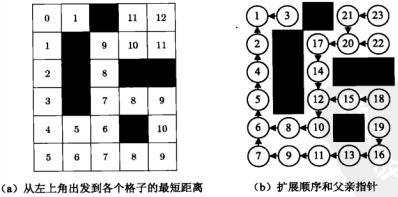
\includegraphics{maze.png}\\
\figcaption{用BFS求迷宫中最短路径}\label{fig:maze}
\end{center}

\subsubsection{代码}
\begin{Codex}[label=maze.c]
#include <stdio.h>
#include <string.h>

#define MAXN 100

// 迷宫的行数,列数
static int n, m;
// 迷宫,0表示空地,1表示障碍物
static int G[MAXN][MAXN];
// 标记格子是否已访问过
static int visited[MAXN][MAXN];
// 每个格子的前驱
static int father[MAXN][MAXN];
// 前趋到该格子的前进方向
static int last_direction[MAXN][MAXN];

// 四个方向
static const char name[4] = {'U','R','D','L'};
static const int dx[4] = {-1, 0, 1, 0}; // 行
static const int dy[4] = {0, 1, 0, -1}; // 列

// 队列
static int q[MAXN * MAXN];

/*
 * @brief 广搜
 *
 * @param[in] x 入口的x坐标
 * @param[in] y 入口的y坐标
 * @return 无
 */
static void bfs(int x, int y) {
    int front = 0, rear = 0;
    int u = x * m + y;
    int d; // 方向
    
    father[x][y] = u; // 打印路径时的终止条件
    visited[x][y] = 1;// 千万别忘记了标记此处的访问记录
    q[rear++] = u;
    while (front < rear) {
        u = q[front++];
        x = u / m;	y = u % m;
        for(d = 0; d < 4; d++) { // 代表四个方向
            const int nx = x + dx[d];
            const int ny = y + dy[d];
            
            if (nx >= 0 && nx < n && ny >= 0 && ny < m &&  // //(nx, ny)没有出界
                !G[nx][ny] && !visited[nx][ny]) { // 不是障碍且没被访问过
                const int v = nx * m + ny;
                q[rear++] = v;
                father[nx][ny] = u; // 记录(nx, ny)的前趋
                visited[nx][ny] = 1; // 访问记录
                last_direction[nx][ny] = d; // 记录从(x, y)到(nx, ny)的方向
            }
        }
    }
}

/*
 * @brief 递归实现路径输出
 *
 * 如果格子(x, y)有父亲(fx, fy),需要先打印出从入口到(fx, fy)的最短路径,然后再
 * 打印从 (fx, fy)到 (x,y) 的移动方向。
 *
 * @param[in] x 目标点的x坐标
 * @param[in] y 目标点的y坐标
 * @return 无
 */
static void print_path_r(const int x, const int y) {
    const int fx = father[x][y] / m;
    const int fy = father[x][y] % m;
    if (fx != x || fy != y) {
        print_path_r(fx, fy);
        putchar(name[last_direction[x][y]]);
    }
}

static int direction[MAXN * MAXN];
/*
 * @brief 显式栈实现路径输出
 *
 * @param[in] x 目标点的x坐标
 * @param[in] y 目标点的y坐标
 * @return 无
 */
static void print_path(int x, int y) {
    int c = 0;
    while(1) {
        const int fx = father[x][y] / m;
        const int fy = father[x][y] % m;
        if (fx == x && fy == y) break;
        direction[c++] = last_direction[x][y];
        x = fx;
        y = fy;
    }
    while (c--) {
        putchar(name[direction[c]]);
    }
}

/*
Sample Input
6 5
00100
01000
01011
01000
00010
00000
Sample Output
(0,0)-->(0,4), DDDDRRUUURUR
*/
int main(void) {
    int i, j;
    char s[MAXN];

    scanf("%d%d", &n, &m);

    for(i = 0; i < n; i++) {
        scanf("%s", s);
        for(j = 0; j < m; j++) {
            G[i][j] = s[j] - '0';
        }
    }

    printf("从入口到出口迷宫路径:\n");
    bfs(0, 0);	// (0, 0)是入口
    print_path(0, 4); // (0, 4) 是出口
    printf("\n");
    return 0;
}
\end{Codex}

\subsubsection{类似的题目}
与本题相同的题目:
\begindot
\item 《算法竞赛入门经典》\footnote{刘汝佳,算法竞赛入门经典,清华大学出版社,2009}第108页6.4.2节
\item  POJ 3984 - 迷宫问题, \myurl{http://poj.org/problem?id=3984}
\myenddot

与本题相似的题目:
\begindot
\item  POJ 2049 - Finding Nemo, \myurl{http://poj.org/problem?id=2049}
\myenddot

\subsection{八数码问题}
\label{subsec:eightDigits}
编号为1$\sim$8的8个正方形滑块摆成3行3列,有一个格子空着,如图~\ref{fig:eightDigits}所示。

\begin{center}
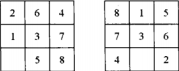
\includegraphics{eight-digits.png}\\
\figcaption{用BFS求迷宫中最短路径}\label{fig:eightDigits}
\end{center}

每次可以把与空格相邻的滑块(有公共边才算相邻)移到空格中,而它原
来的位置就成了新的空格。目标局面固定如下(用$x$表示空格):\\
1 2 3 \\
4 5 6 \\
7 8 x

给定初始局面,计算出最短的移动路径。

\textbf{输入}

用一行表示一个局面,例如下面的这个局面: \\
 1  2  3 \\
 x  4  6 \\
 7  5  8 \\
可以表示为 1 2 3 x 4 6 7 5 8。 

\textbf{输出}

如果有解答,输出一个由四个字母'r','l','u','d'组成的移动路径。
如果没有,输出"unsolvable"。 

\textbf{样例输入} \\
2  3  4  1  5  x  7  6  8

\textbf{样例输出} \\
ullddrurdllurdruldr

\subsubsection{分析}
计算“最短”,很自然的想到BFS。

怎么判断一个状态已经访问过?用哈希表或者集合。哈希表的话,由于C++ STL 还没有 \fn{std::hashset},
需要自己实现哈希表,然后由于本题的特殊性,存在一种完美哈希(perfect hashing)方案。集合可以直接
使用\fn{std::set}。总结起来,有以下三个方法:
\begindot
\item 把排列变成整数,这是一种完美哈希,即不存在冲突
\item 用普通的哈希表,这种方法通用一些,速度也略慢。手工实现哈希表,把哈希值相同的组成一个单链表,
\item 用 \fn{std::set} 实现判重,代码最短,速度也最慢(本题用这个方法会TLE)。建议把该方法作为“跳板”,
先写一个STL版的程序,确保主算法正确,然后把\fn{std::set}替换成自己写的哈希表。
\myenddot

此题更优的解法还有双向BFS(见\S \ref{sec:biBFS}),A*算法(见\S \ref{sec:astar})。

\subsubsection{代码}
\begin{Codex}[label=eight_digits_bfs.c]
#include<stdio.h>
#include<string.h>

#define DIGITS 9 // 棋盘中数字的个数,也是变进制数需要的位数
#define     MATRIX_EDGE 3       // 棋盘边长

// 3x3的棋盘,状态最多有 9!种
#define     MAX         362880

typedef int State[DIGITS]; // 单个状态

static State q[MAX]; // 队列,也是哈希表
static int front, rear;
static int dist[MAX - 1]; // 由初始状态到本状态的最短步数
static int father[MAX - 1]; // 父状态,初始状态无父状态
static char move[MAX - 1]; // 父状态到本状态的移动方向

// 目标状态
static const int goal[] = {1, 2, 3, 4, 5, 6, 7, 8, 0};
static const int space_number = 0; // 空格对应着数字 0

// 上下左右四个方向
static const int dx[] = {-1, 1, 0, 0};
static const int dy[] = {0, 0, -1, 1};
static const char dc[] = { 'u', 'd', 'l', 'r' };

/**
 * @brief 初始化哈希表.
 * @return 无
 */
static void init_lookup_table(); // 版本 1

/**
 * @brief 插入到 visited表中.
 * @param[in] index 状态在队列中的位置
 * @return 成功返回1,失败返回0
 */
static int try_to_insert(const int index);

static void init_lookup_table_hash(); // 版本2
static int try_to_insert_hash(const int index);

static void init_lookup_table_stl(); // 版本3
static int try_to_insert_stl(const int index);

/**
 * @brief 单向BFS.
 * @return 返回目标状态在队列q中的下标 ,失败则返回0
 */
static int bfs() {
    // 三个版本随意切换
    init_lookup_table(); // 初始化一个节点查找表
    // init_lookup_table_hash();
    // init_lookup_table_stl(); // 这个版本会 Time Limit Exceeded
    
    father[0] = 0; // 初始状态无父状态
    dist[0] = 0;
    move[0] = -1;

    while (front < rear) {
        int x, y, z, d;
        const State* const s = &(q[front]);
        if (memcmp(goal, (*s),sizeof((*s))) == 0) {
            return front;  // 找到目标状态,成功返回
        }
        for (z = 0; z < 9; z++)  if ((*s)[z] == space_number) {
            break;  // 找 0 的位置
        }
        
        x=z / MATRIX_EDGE, y=z % MATRIX_EDGE; // 获取行列编号
        for (d=0; d < 4; d++) {  // 向四个方向扩展
            const int newx = x + dx[d];
            const int newy = y + dy[d];
            const int newz = newx * MATRIX_EDGE + newy;

            if (newx >= 0 && newx < MATRIX_EDGE && newy >= 0 &&
                newy < MATRIX_EDGE) { // 没有越界
                State * const t = &(q[rear]);
                memcpy(t, s, sizeof((*s)));
                (*t)[newz] = (*s)[z];
                (*t)[z] = (*s)[newz];

                // 三个版本随意切换
                if (try_to_insert(rear)) { // 利用查找表判重
                // if (try_to_insert_hash(rear)) {
                // if (try_to_insert_stl(rear)) {
                    father[rear] = front;
                    move[rear] = dc[d];
                    dist[rear] = dist[front] + 1;
                    rear++;
                } 
            }
        }

        front++;
    }

    return 0;//失败 
}


/**
 * @brief 输入.
 * @return 无
 */
static void input() {
    int ch, i;
    for (i = 0; i < DIGITS; ++i) {
        do {
            ch = getchar();
        } while ((ch != EOF) && ((ch < '1') || (ch > '8')) && (ch != 'x'));
        if (ch == EOF) return;
        if (ch == 'x') q[0][i] = 0; // x 映射成数字 0
        else           q[0][i] = ch - '0';
    }
    return;
}

static int top = -1;
static char stack[MAX];
/**
 * @brief 打印从初始状态到目标状态的移动序列.
 * @param[in] index 目标状态在队列q中的下标
 * @return 无
 */
static void output(const int index) {
    int i;
    for (i = index; i > 0; i = father[i]) {
        stack[++top] = move[i];
    }
    for (i = top; i >= 0; --i) {
        printf("%c", stack[i]);
    }
    printf("\n");
}

int main() {
    int ans;

    front = 0; rear = 1;
    input();
    
    ans = bfs();
    if ( ans > 0) {
        output(ans);
    } else {
        printf("no solution\n");
    }
    return 0;
}

/***********************方案1 把排列变成整数**************************/
// 9 位变进制数(空格)能表示0到(9!-1)内的所有自然数,恰好有9!个,
// 与状态一一对应,因此可以把状态一一映射到一个9位变进制数

// 9 位变进制数,每个位数的单位,0!~8!
static const int fac[] = {40320, 5040, 720, 120, 24, 6, 2, 1, 1};

// 采用本方案,由于是完美哈希,没有冲突,
// 可以用 MAX 代替 MAX_HASH_SIZE,减少内存占用量
static int visited[MAX]; // 历史记录表

/** 初始化哈希表. */
static void init_lookup_table() {
    memset(visited, 0, sizeof(visited));
}

/**
 * @brief 计算状态的hash值,这里用康托展开,是完美哈希.
 *
 * @param[in] s 状态
 * @return 序数,作为hash值
 */
static int hash(const State s) {
    int i, j;
    int key = 0; // 将 q[index] 映射到整数 key
    for (i = 0; i < 9; i++) {
        int cnt = 0;
        for (j = i + 1; j < 9; j++) if (s[i] > s[j]) cnt++;
        key += fac[i] * cnt;
    }
    return key;
}

/**
 * @brief 插入到 visited表中.
 * @param[in] index 状态在队列中的位置
 * @return 成功返回1,失败返回0
 */
static int try_to_insert(const int index) {
    const int key = hash(q[index]); // 将 q[index] 映射到整数 code
    
    if (visited[key]) return 0;
    else visited[key] = 1;

    return 1;
}

/**************************方案2 哈希表**********************************/
#define MAX_HASH_SIZE  1000000  // 状态的哈希表容量,比 9! 大即可

int head[MAX_HASH_SIZE];
int next[MAX];

static void init_lookup_table_hash() {
    memset(head, 0, sizeof(head));
    memset(next, 0, sizeof(next));
}
static int hash2(const State *s) {
    int i;
    int v = 0;
    for(i = 0; i < 9; i++) v = v * 10 + (*s)[i];
    return v % MAX_HASH_SIZE;
}

static int try_to_insert_hash(const int index) {
    const int h = hash2(&(q[index]));
    int u = head[h]; // 从表头开始查找单链表
    while(u) {
        // 找到了,插入失败
        if(memcmp(q[u], q[index], sizeof(State)) == 0) return 0;
        u = next[u]; // 顺着链表继续找
    }
    next[index] = head[h]; // 插入到链表中
    head[h] = index; // head[h]和 next[index] 组成了一个节点
    return 1;
}

/****************************方案3 STL************************************/
#include <set>
struct cmp {
    bool operator() (int a, int b) const {
        return memcmp(&q[a], &q[b], sizeof(State)) < 0;
    }
};
std::set<int, cmp> visited_set;

void init_lookup_table_stl() { visited_set.clear(); }

int try_to_insert_stl(const int index) {
    if (visited_set.count(index)) return 0;
    visited_set.insert(index);
    return 1;
}
\end{Codex}

\subsubsection{类似的题目}
与本题相同的题目:
\begindot
\item 《算法竞赛入门经典》\footnote{刘汝佳,算法竞赛入门经典,清华大学出版社,2009} 第131页7.5.3节
\item  POJ 1077 - Eight, \myurl{http://poj.org/problem?id=1077}
\myenddot

与本题相似的题目:
\begindot
\item  POJ 2893 - M × N Puzzle, \myurl{http://poj.org/problem?id=2893}
\myenddot

\section{双向BFS} %%%%%%%%%%%%%%%%%%%%%%%%%%%%%%
\label{sec:biBFS}
\subsection{八数码问题}
题目见 \S \ref{subsec:eightDigits}。

\textbf{代码}

\begin{Codex}[label=eight_digits_bibfs.c]
\end{Codex}

\section{最小生成树} %%%%%%%%%%%%%%%%%%%%%%%%%%%%%%

\subsection{Prim算法}

\subsection{Kruskal算法}

\section{最短路径} %%%%%%%%%%%%%%%%%%%%%%%%%%%%%%

\subsection{单源最短路径(Dijkstra算法)}

\subsection{每点最短路径(Floyd算法)}

\section{拓扑排序} %%%%%%%%%%%%%%%%%%%%%%%%%%%%%%

\section{关键路径} %%%%%%%%%%%%%%%%%%%%%%%%%%%%%%

\section{A*算法} %%%%%%%%%%%%%%%%%%%%%%%%%%%%%%
\label{sec:astar}

\subsection{八数码问题}
题目见 \S \ref{subsec:eightDigits}。

\subsubsection{代码}
\begin{Codex}[label=eight_digits_astar.c]
/**
 简单解释几个要点,便于理解代码.
 1. 怎么判断是否有解?只要计算出的逆序个数总和为奇数,该数据必然无解
 2. 如何判断某一状态是否到过?本题存在一种完美哈希方案,即用康托展开。
    详见 http://128kj.iteye.com/blog/1699795
    2.1.将一个状态视为数字 0-8 的一个排列,将此排列转化为序数,作为此状
 态的 HASH 值。0表示空格.转化算法此处不再赘述。

    2.2.排列转化为序数,用序数作为hash值
    例,1 2 3 这三个数字的全排列,按字典序,依次为
 123 -- 0
 132 -- 1
 213 -- 2
 231 -- 3
 312 -- 4
 321 -- 5
 其中,左侧为排列,右侧为其序数。
 
 3.使用数据结构 堆 加速挑选最优值。
 
 4.函数 g 的计算,此状态在搜索树中已经走过的路径的节点数.
 
 5.估价函数 h ,采用曼哈顿距离, 见代码 calcH 函数。曼哈顿距离的定义是,
 假设有两个点(x1,y1),(x2,y2),则曼哈顿距离L1=|x1-x2| + |y1-y2|
 */

#include <stdio.h>
#include <string.h>
#include <stdlib.h>

// 3x3的棋盘,状态最多有 9!种
// 8位变进制数(空格)能表示0到(9!-1)内的所有自然数,恰好有9!个,
// 与状态一一对应,因此可以把状态一一映射到一个8位变进制数
#define     MAX         362880

#define DIGITS 9 // 棋盘中数字的个数,也是变进制数需要的位数
#define     MATRIX_EDGE 3       // 棋盘边长

#define     MOD         10      // 按十取模

typedef struct {
    int state; // 状态
    int parent;     // 父状态
    int flag;   // -1 表示已经展开过了closed,0表示死节点,1 表示还未展开, open
    int g, h, f; // 三个评估函数
    char choice;  // 左右上下四个方向移动,见全局常量 DI DJ DC
} state_t;

static state_t states[MAX];  // 全局的一条状态变化路径

static int  startIndex, goalIndex; // 开始状态,目标状态对应的hash值

// 目标状态
static const int goal = 123456780;
// 每个数字在棋盘中的位置,例如0,在(1,1)=4这个位置上
static const int goal_pos[DIGITS] = {8,0,1,2,3,4,5,6,7};
static const int space_number = 0; // 空格对应着数字 0

// 上下左右四个方向
static const int DI[] = {-1, 1, 0, 0};
static const int DJ[] = {0, 0, -1, 1};
static const char DC[] = { 'u', 'd', 'l', 'r' };

// 9 位变进制数,每个位数的单位,0!~8!
static const int fac[] = {40320, 5040, 720, 120, 24, 6, 2, 1, 1};

/**
 * @brief 计算状态的hash值,这里用康托展开,是完美哈希.
 *
 * @param[in] s 当前状态
 * @return 序数,作为hash值
 */
static int hash(int s) {
    int i, j;
    int d[DIGITS];
    int key = 0;

    for(i = DIGITS - 1; i >=0; i--) {
        d[i] = s % MOD;
        s /= MOD;
    }
    
    for (i = 0; i < DIGITS; i++) {
        int c = 0; // 逆序数
        for (j = i + 1; j < DIGITS; j++) {
            if(d[j] < d[i]) {
                c++;
            }
        }
        key += c * fac[i];
    }
    
    return key;
}

// 堆
static int heap[MAX + 4], heapIndex[MAX + 4], heapN;

static void heapUp(int j) {
    int i = j / 2;
    const int x = heap[j];
    while (i > 0) {
        if (states[heap[i]].f <= states[x].f) break;
        heapIndex[heap[j] = heap[i]] = j;
        j = i;
        i = j / 2;
    }
    heapIndex[heap[j] = x] = j;
}

static void heapDown(int i) {
    int j = i + i;
    const int x = heap[i];
    while (j <= heapN) {
        if ((j < heapN) && (states[heap[j]].f >
            states[heap[j + 1]].f)) ++j;
        if (states[x].f <= states[heap[j]].f) break;
        heapIndex[heap[i] = heap[j]] = i;
        i = j;
        j = i + i;
    }
    heapIndex[heap[i] = x] = i;
}

static int heapPop() {
    const int x = heap[1];
    heapIndex[heap[1] = heap[heapN--]] = 1;
    if (heapN > 1) {
        heapDown(1);
    }
    return x;
}

static void heapAdd(const int x) {
    ++heapN;
    heapIndex[heap[heapN] = x] = heapN;
    heapUp(heapN);
}

/**
 * 估价函数h。
 * @param s 状态
 * @return 预估代价
 */
static int calcH(int s) {
    int i;
    int h = 0;
    
    for (i = DIGITS - 1; i >= 0; --i) {
        const int p = s % 10;
        s /= 10;
        // 曼哈顿距离
        h += abs(i / MATRIX_EDGE - goal_pos[p] / MATRIX_EDGE) +
            abs(i % MATRIX_EDGE - goal_pos[p] % MATRIX_EDGE);
    }
    return h;
}

/**
 * @brief 输入.
 * @return  成功返回数字,失败返回0
 * @remark 《算法竞赛入门经典》第131页7.5.3节,是用0表示空格,
 * POJ 1077是用'x'表示空格,前者简化了一点,POJ 1077还需要把'x'映射成0
 */
static int input() {
    int ch, i;
    int start = 0;
    for (i = 0; i < DIGITS; ++i) {
        do {
            ch = getchar();
        } while ((ch != EOF) && ((ch < '1') || (ch > '8')) && (ch != 'x'));
        if (ch == EOF) return 0;
        if (ch == 'x') start = start * MOD + space_number; // x 映射成数字 0
        else             start = start * MOD + ch - '0';
    }
    return start;
}

/**
 * 计算一个排列的逆序数,0 除外.
 */
static int inversion_count(int permutation) {
    int i, j;
    int d[DIGITS];
    int c = 0; // 逆序数

    for(i = DIGITS - 1; i >=0; i--) {
        d[i] = permutation % MOD;
        permutation /= MOD;
    }
    
    for (i = 1; i < DIGITS; i++)  if (d[i] != space_number) {
        for (j = 0; j < i; j++) {
            if(d[j] != space_number) {
                if (d[j] > d[i]) {
                    c++;
                }
            }
        }
    }
    return c;
}

/**
 * 判断是否无解.
 *
 * 求出除0之外所有数字的逆序数之和,也就是每个数字后面比它小的数字的个数的和,
 * 称为这个状态的逆序。若两个状态的逆序奇偶性相同,则可相互到达,否则不可相互到达。
 * 由于原始状态的逆序数为0(偶数),因此逆序数为偶数的目标状态有解。
 *
 * @param s 目标状态
 * @return 1表示无解,0表示有解
 */
static int not_solvable(const int s) {
    return inversion_count(s) % 2;
}


static char choice[4];
static int nextIndex[4];
// 向四个方向扩展
static void next(int s) {
    int i, j, k;
    static int p[MATRIX_EDGE][MATRIX_EDGE]; // 一个状态对应的矩阵
    int i0, j0;  // 空格位置

    for (i = MATRIX_EDGE - 1; i >= 0; i--) {
        for (j = MATRIX_EDGE - 1; j >= 0; j--) {
            p[i][j] = s % MOD;
            s /= MOD;
            if (p[i][j] == space_number) {
                i0 = i;
                j0 = j;
            }
        }
    }
    // 向四个方向探索
    for (k = 0; k < 4; ++k) {
        const int sx = i0 + DI[k]; // 空格的新位置(sx, sy)
        const int sy = j0 + DJ[k];
        if ((sx >= 0) && (sx < 3) && (sy >= 0) && (sy < 3)) {
            int key;
            p[i0][j0] = p[sx][sy];
            p[sx][sy] = space_number;
            // 移动空格后,计算新的状态
            s = 0;
            for (i = 0; i < MATRIX_EDGE; i++)
                for (j = 0; j < MATRIX_EDGE; j++)
                    s = s * MOD + p[i][j];
            p[sx][sy] = p[i0][j0]; // 将矩阵还原,(i0, j0)可以不管
            
            key = nextIndex[k] = hash(s);
            choice[k] = DC[k];
            if (states[key].state == 0) { // 该状态还没有出现过
                states[key].state = s;
                states[key].h = calcH(s);
            }
        } else {// 越界了
            nextIndex[k] = -1;
        }
    }
}

/**
 * @brief A*搜索
 * @param[in] start 初始状态
 * @return 如果无解,返回0,如果有解返回1
 */
static int astar(const int start) {
    int i, j, k, ng, nf;
    if (not_solvable(start)) return 0;

    startIndex = hash(start);
    goalIndex  = hash(goal);
    if (start == goal) return 1;
    
    memset(states, 0, sizeof(states));
    states[startIndex].state = start;
    states[startIndex].flag    = 1;
    states[startIndex].g       = 0;
    states[startIndex].h       = states[startIndex].f = calcH(start);
    heapN = 0;
    heapAdd(startIndex);
    while (heapN > 0) {
        i = heapPop();
        if (i == goalIndex) return 1; // 找到目标,返回

        states[i].flag = -1;
        ng = states[i].g + 1;
        next(states[i].state);
        for (k = 0; k < 4; ++k) {
            j = nextIndex[k];
            if (j < 0) continue;
            nf = ng + states[j].h;
            if ((states[j].flag == 0) || ((states[j].flag == 1) &&
                (nf < states[j].f))) {
                states[j].parent = i;
                states[j].choice = choice[k];
                states[j].g    = ng;
                states[j].f    = nf;
                if (states[j].flag > 0) {
                    heapUp(heapIndex[j]);
                    heapDown(heapIndex[j]);
                } else {
                    heapAdd(j);
                    states[j].flag = 1;
                }
            }
        }
    }
    return 0;
}

static int top = -1;
static char stack[MAX];
/**
 * @brief 打印移动序列.
 * @return 无
 */
static void output() {
    int i;
    for (i = goalIndex; i != startIndex; i = states[i].parent) {
        stack[++top] = states[i].choice;
    }
    for (i = top; i >= 0; --i) {
        printf("%c", stack[i]);
    }
    printf("\n");
}

int main_astar() {
    const int start = input();
    if (start > 0) {
        if (astar(start)) {
            output();
        } else {
            printf("no solution\n");
        }
    }
    return 0;
}
\end{Codex}
